\documentclass[a4paper, 12pt]{article}

% -- Language --
\usepackage[spanish]{babel}
\usepackage[utf8]{inputenc}

% ----- Fonts -----
% -- Color --
\usepackage{xcolor}
%\definecolor{azul}{RGB}{00,33,99}
\definecolor{azul}{RGB}{35,72,180}

% -- Page Margin --
\usepackage[margin=1in]{geometry}

% -- Espaciados --
\newcommand{\Pspace}{0.5cm}
\newcommand{\Aspace}{0.2cm}

% -- Imagenes --
\usepackage{graphicx}

% -- Matemáticas --
\usepackage{amsmath, amssymb}

% -- Gráficas --
\usepackage{pgfplots}
\pgfplotsset{compat=1.18}

% -- Código --
\usepackage{listings}
\lstset{
    language=C++,                   % Lenguaje del código
    basicstyle=\ttfamily\small,     % Fuente del código
    keywordstyle=\color{blue},      % Color de palabras clave
    commentstyle=\color{gray},      % Color de comentarios
    stringstyle=\color{red},        % Color de cadenas
    numbers=left,                   % Números de línea a la izquierda
    numberstyle=\tiny\color{gray},
    breaklines=true,                % Permitir saltos de línea
    frame=single                    % Marco alrededor del código
}


\title
{
    Probabilidad 2025-1 \\
    Tareas Parcial 3
    }

    \begin{document}

    \maketitle

    \begin{center}
        \begin{tabular}{r|l}
            \textbf{Expediente} & \textbf{Nombre} \\ \hline
            219208106 & Bórquez Guerrero Angel Fernando \\
            223203899 & Tostado Cortes Dante Alejandro \\
        \end{tabular}
    \end{center}

    \rule{\linewidth}{0.3mm}



    % ---------- Tarea 9 ----------
    \vspace{0.3cm}

    \begin{center}
        { \LARGE Tarea 9}
    \end{center}

    \begin{enumerate}
        % - Problema 1
        \item Comprobar si la siguiente función es de probabilidad \par
        \[
            f(x) =
            \begin{cases}
                \frac{1 / 2}{\sqrt{x}} & 0 < x < 1 \\
                0 & \text{Otro caso}
            \end{cases}
        \]
            % Respuesta:
            \vspace{\Aspace}
            { \color{azul} 
                \[  \int_{0}^{1}\frac{\frac{1}{2}}{\sqrt{x}}dx 
                    = \frac{1}{2} \int_{0}^{1}x^{-\frac{1}{2}}dx
                    = \frac{1}{2} \left[ \frac{\sqrt{x}}{\frac{1}{2}} \Big|_{0}^{1} \right]
                    = \sqrt{x} \Big|_{0}^{1}
                    = \sqrt{1} - \sqrt{0} = 1
                \]
            }
        
        \newpage
        % - Problema 2
        \vspace{\Pspace}
        \item Encontrar la función de distribución con la función de probabilidad
        \[
            f(x) =
            \begin{cases}
                2x & 0 \leq x \leq 1 \\
                0 & \text{Otro caso}
            \end{cases}
        \]       
        Grafica ambas funciones

            % Respuesta:
            \vspace{\Aspace} \par
            { \color{azul} 
                Función de probabilidad: \par
                \begin{tikzpicture}
                \begin{axis}
                [
                    axis lines = middle,
                    xlabel = $x$,
                    ylabel = {$f(x)$},
                    samples=100,
                    xmin=-0.5, xmax=1.5,
                    ymin=-0.5, ymax=2.5
                ]
                
                % Primera parte: f(x) = 2x para 0 <= x <= 1
                \addplot[color=blue, thick, domain=0:1]{2*x};

                % Segunda parte: f(x) = 0 en otros casos
                \addplot[color=red, thick, domain=-0.5:0]{0};
                \addplot[color=red, thick, domain=1:1.5]{0};

                % Punto cerrado en (0,0)
                \addplot[only marks, mark=*, mark size=2pt, color=blue] coordinates {(0,0)};

                % Punto cerrado en (1,2)
                \addplot[only marks, mark=*, mark size=2pt, color=blue] coordinates {(1,2)};
                \end{axis}
                \end{tikzpicture}

                Función de distribución:
                \[
                    F(x) = \int_{-\infty}^{x} 2u du
                    = 2 \int_{-\infty}^{x} u du =
                    \begin{cases}
                        0 & x < 0 \\
                        x^{2} & 0 \leq x \leq 1 \\
                        1 & x > 1                       
                    \end{cases}
                \]
                \begin{tikzpicture}
                \begin{axis}
                [
                    axis lines = middle,
                    xlabel = $x$,
                    ylabel = {$F(x)$},
                    samples=100,
                    xmin=-0.5, xmax=1.5,
                    ymin=-0.5, ymax=2.5
                ]
                
                % Primera parte: f(x) = 2x para 0 <= x <= 1
                \addplot[color=blue, thick, domain=0:1]{x^2};

                % Segunda parte: f(x) = 0 en otros casos
                \addplot[color=red, thick, domain=-0.5:0]{0};
                \addplot[color=red, thick, domain=1:1.5]{1};

                % Punto cerrado en (0,0)
                \addplot[only marks, mark=*, mark size=2pt, color=blue] coordinates {(0,0)};

                % Punto cerrado en (1,1)
                \addplot[only marks, mark=*, mark size=2pt, color=blue] coordinates {(1,1)};
                \end{axis}
                \end{tikzpicture}
            }

        \newpage
        % - Problema 3
        \item Sea la función de distribución
        \[
            F(x) =
            \begin{cases}
                0 & x < 0 \\
                x & 0 \leq x \leq 1 \\
                1 & x > 1
            \end{cases}
        \]
        Determinar si se trata de la función de distribución de una variable aleatoria discreta o continua. Encontrar además la correspondiente función de probabilidad o densidad y graficarlas.
    \end{enumerate}



    % ---------- Tarea 6 ----------
    \newpage
    \begin{center}
        { \LARGE Tarea 6}
    \end{center}

    \begin{enumerate}
        %  - Problema 1
        \item Un dado equilibrado se lanza dos veces consecutivas. Sea $X$ la diferencia entre el resultado del primer y el segundo lanzamiento.
            % Respuestas:
            \vspace{\Aspace} \par
            a) Encuentre la función de probabilidad de $X$.
            \\ { \color{azul} $f(x) = P[X = x] = \frac{6 - |x|}{36}$ }

            \vspace{\Aspace} \par
            b) Encuentre la función de distribución de $X$.
            \\ { \color{azul} $F(x) = \sum\limits_{x = -5}^{5} \frac{6 - |x|}{36}$ }

            \vspace{\Aspace} \par
            c) Determinar el valor esperado de $X$.
            \\ { \color{azul} $E[X] = \mu = \sum\limits_{x = -5}^{5} x\frac{6 - |x|}{36} = 0$ }

            \vspace{\Aspace} \par
            d) Determinar la varianza de $X$.
            \\ { \color{azul} $Var(X) = \sigma^{2} = \sum\limits_{x = -5}^{5} (x - \mu)^{2} (\frac{6 - |x|}{36}) = \frac{35}{6}$ }

            \vspace{\Aspace} \par
            e) Determinar el histograma.
            \begin{figure}[h]
                \centering
                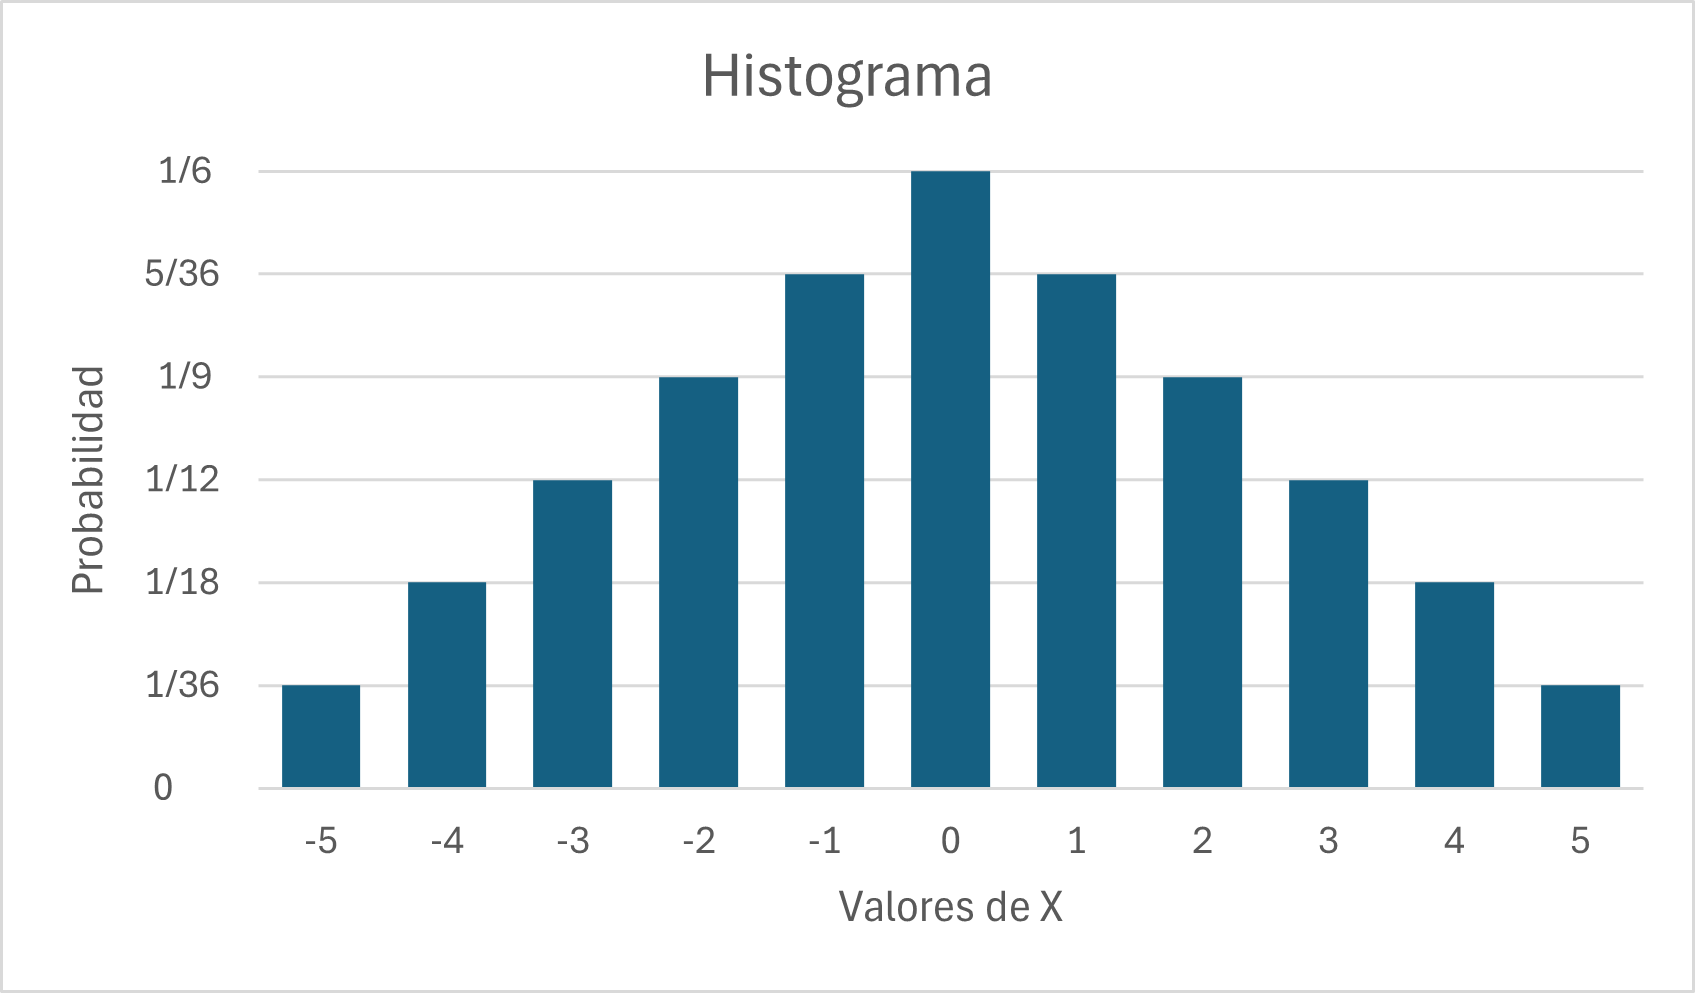
\includegraphics[width=0.6\textwidth]{./Assets/HistogramaT6P1.png}
            \end{figure}

            f) Dibujar el valor esperado y el intervalo que resulta de estar dentro de una desviación estándar de la media.
            \vspace{\Aspace}
            \\ { \color{azul} $\sigma = \sqrt{\frac{35}{6}}$ }
            \begin{figure}[h]
                \centering
                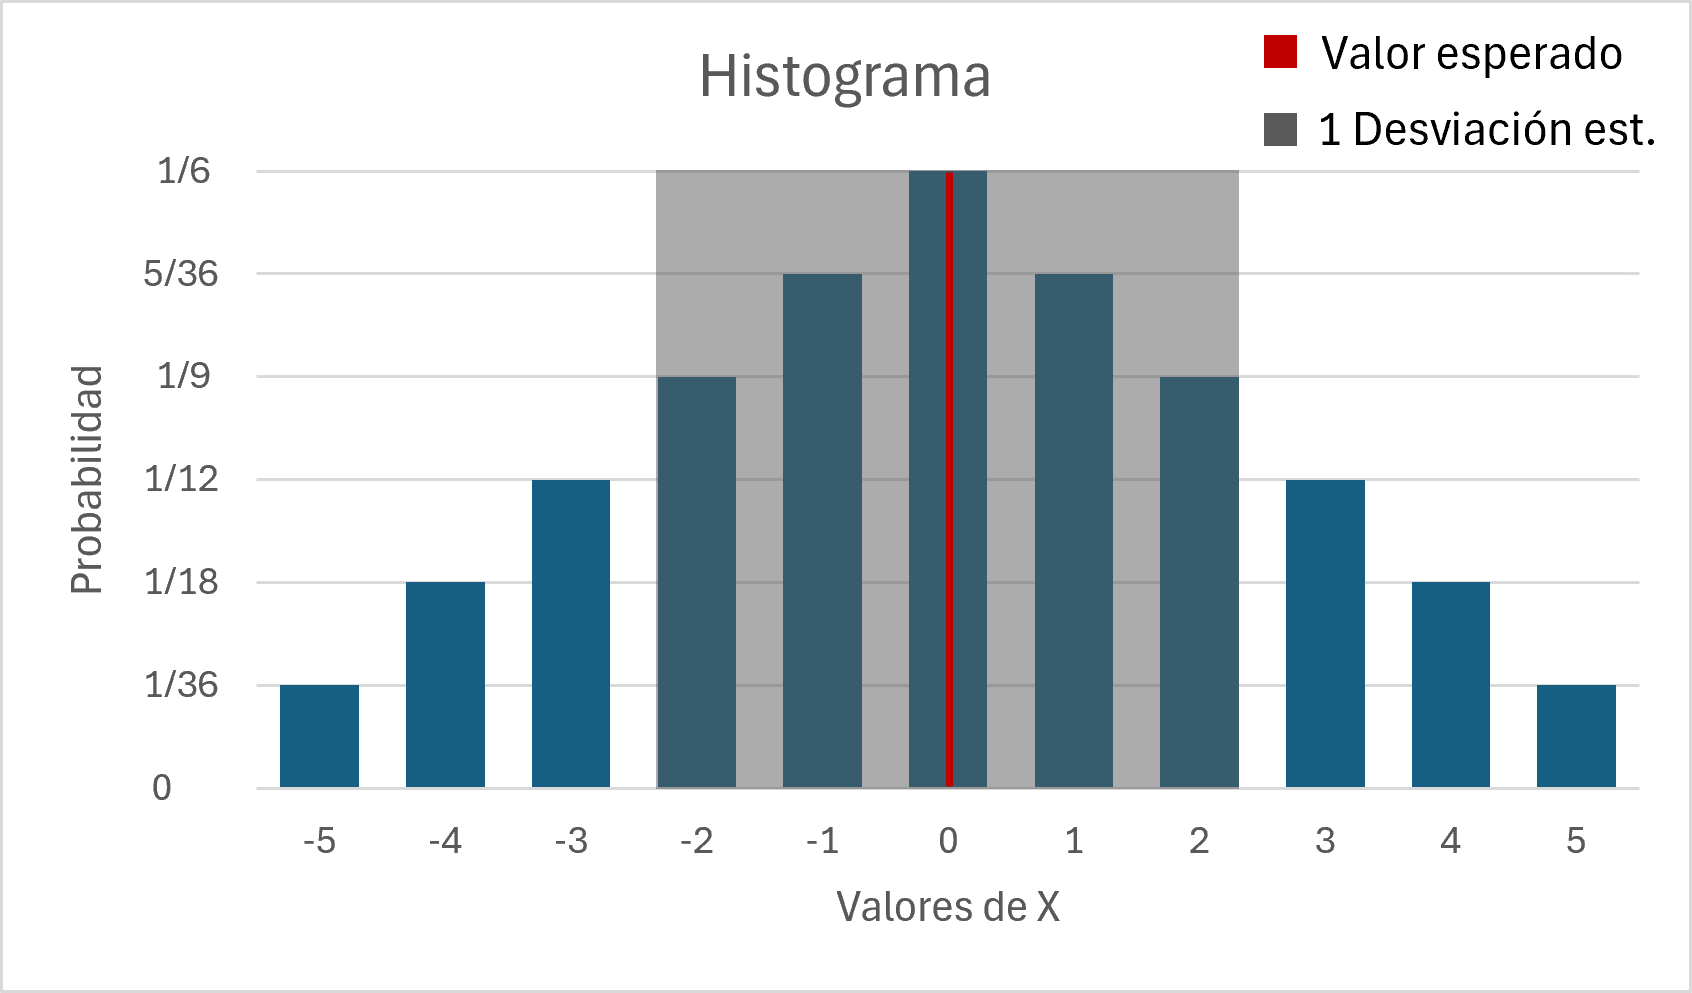
\includegraphics[width=0.6\textwidth]{./Assets/Histograma2T6P1.png}
            \end{figure}

            \newpage
            % - Problema 2
            \vspace{\Pspace}
        \item Se sabe que un jugador tiene una probabilidad del 95\% de ganar un juego importante. Sea $X$ la variable aleatoria que indica si gana o pierde el juego.
            % Respuestas:
            \vspace{\Aspace} \par
            a) ¿Sigue una distribución de Bernoulli?
            \\ { \color{azul} Dado que solo existen dos posibles resultados (éxito o fracaso), esta sigue una distribución de Bernoulli $X \sim Be(0{.}95)$ }

            \vspace{\Aspace} \par
            b) Si puediera jugar muchas veces el juego importante, ¿qué porcentaje de victorias esperaría observar?
            \\ { \color{azul} Si cada juego es independiente, $E[X] = 0{.}95 = 95\%$ }

            \vspace{\Aspace} \par
            c) ¿Cuál es la varianza de esta variable aleatoria?
            \\ { \color{azul} $Var(X) = \sigma^2 = 0{.}95 (1 - 0{.}95) = 0{.}0475$ }

            \vspace{\Aspace} \par
            d) Determine el intervalo de valores que están dentro de una desviación estándar de la media.
            \\ { \color{azul}
            $\sigma = \sqrt{0.0475} = \frac{\sqrt{19}}{20} = 0{.}218$ \vspace{0.1cm}
            \newline $[E[X]] - \sigma, E[X] + \sigma] = [0{.}95 - 0{.}218, 0{.}95 + 0{.}218] = [0{.}732, 1{.}168]$ \vspace{0.1cm}
            \newline Dado que no pueden haber valores mayores que 1, el intervalo termina siendo $[0{.}732, 1]$
            }
    \end{enumerate}



    % ---------- Tarea 7 ----------
    \newpage
    \begin{center}
        { \LARGE Tarea 7}
    \end{center}

    \begin{enumerate}
            %  - Problema 1
        \item Antes de la venta de pianos, deben probarse para saber si se encuentran en buen estado o defectuoso. El porcentaje de defectuosos es de 5\%. Sea $X$ el número de pianos en buen estado en una muestra aleatoria de tamaño $n = 25$,
            % Respuestas:
            \vspace{\Aspace} \par
            a) ¿Qué tipo de distribución tiene $X$?
            \\ { \color{azul} Dado que solo existen dos posibles resultados (buen estado o defectuoso) y contamos con una muestra, esta sigue una distribución binomial $X \sim Bin(25, 0{.}95)$ }

            \vspace{\Aspace} \par
            b) Determinar la probabilidad de observar exactamente 7 pianos en buen estado.
            \\ { \color{azul} $P[X = 7] = \binom{25}{7} (0{.}95)^{7} (0{.}05)^{18} = 1{.}28$x$10^{-18}$ }

            \vspace{\Aspace} \par
            c) Determinar la probabilidad de observar 22 o más pianos en buen estado.
            \\ { \color{azul} $P[X \geq 22] = \sum\limits_{x = 22}^{25} \binom{25}{x} (0{.}95)^{x} (0{.}05)^{25 - x} = 0{.}966$ }

            \vspace{\Aspace} \par
            d) Determinar la probabilidad de observar menos de 22 pianos en buen estado
            \\ { \color{azul} $P[X < 22] = 1 - P[X \geq 22] = 1 - 0{.}966 = 0{.}034$ }

            \vspace{\Aspace} \par
            e) Determinar el número de pianos que espera encontrar en buen estado.
            \\ { \color{azul} $E[X] = (25)(0{.}95) = 23{.}75$ }

            \vspace{\Aspace} \par
            f) Determinar la varianza de $X$.
            \\ { \color{azul} $Var(X) = \sigma^{2} = (25)(0{.}95)(0{.}05) = 1{.}1875$ }


            % - Problema 2
            \vspace{\Pspace}
        \item Una pareja desea tener una niña en su familia. La pareja decide tener hijos hasta que se tenga la primer niña. Suponga que la probabilidad de tener una hija es de 0.25. 
            % Respuestas:
            \vspace{\Aspace} \par
            a) ¿Cuál es la probabilidad de que la familia tenga $x$ niñas?
            \\ { \color{azul} $P[X = x] = (1 - 0{.}25)^{x}(0{.}25)$ }

            \vspace{\Aspace} \par
            b) ¿Cuál es la probabilidad de que la familia tenga cuatro hijos?
            \\ { \color{azul} $(0{.}75)^{3}(0{.}25) = 0{.}1055$ }

            \vspace{\Aspace} \par
            c) ¿Cuál es la probabilidad de que la familia tenga cuando mucho cuatro hijos?
            \\ { \color{azul} $\sum\limits_{x = 0}^{4} (0{.}75)^{x}(0{.}25)$ }

            \vspace{\Aspace} \par
            d) ¿Cuántos hijos esperaría que tenga esta familia?
            \\ { \color{azul} $E[X] = \frac{1}{p} = \frac{1}{0{.}25} = 4$ }

            \vspace{\Aspace} \par
            e) ¿Cuál es la desviación estándar?
            \\ { \color{azul} $Var(X) = \sigma^{2} = \frac{1 - p}{p^{2}} = \frac{0{.}75}{(0{.}25)^{2}} = 12$ }


            \newpage
            % - Problema 3
            \vspace{\Pspace}
        \item Sea $X$ una variable aleatoria tal que $ X \sim U\{1, 2, \dots, n\} $. Demuestre que:
            % Respuestas:
            \vspace{\Aspace} \par
            a) $E(X^{2}) = \frac{(n + 1)(2n + 1)}{6}$
            \\ { \color{azul} 
            Dado que $X$ se distribuye de manera uniforme, esto significa que todos los valores tienen la misma probabilidad de ocurrencia.
            \par • El valor esperado de $X$ se calcula de la siguiente manera:
            \[ E[X] = \frac{1}{n} \sum\limits_{i = 1}^{n} x_{i} \]

            \par • La suma de los primeros $n$ números naturales puede ser calculada de la siguiente forma:
            \[ 1 + 2 + \ldots + n = \frac{n(n + 1)}{2} \]

            \par • Reescribiendo la función obtenemos lo siguiente:
            \[ E[X] = \frac{n + 1}{2} \ \forall X \sim U\{1, 2, \ldots, n\} \]

            \par • Ya que $X^{2}$ se distribuye de la misma forma uniforme, su valor esperado se calcula de la siguiente forma:
            \[ E[X^{2}] = \frac{1}{n} \sum\limits_{i = 1}^{n} x_{i}^2 \]

            \par • También podemos calcular la suma de los primeros $n^{2}$ naturales con la siguiente función:
            \[ f(n) = \frac{n(n + 1)(2n + 1)}{6} \ \forall n \in \mathbb{N} \]

            \par • Reescribiendo en la función del valor esperado hemos obtenido lo que deseábamos demostrar.
            \[ E[X^{2}] = \frac{1}{n} \frac{n(n + 1)(2n + 1)}{6} = \frac{(n + 1)(2n + 1)}{6} \]
            }

            \newpage
            \vspace{\Aspace} \par
            b) $Var(X) = \frac{n^{2} - 1}{12}$ 
            \\  { \color{azul} 
            La varianza de una distribución uniforme se calcula de la siguiente forma:
            \[ Var(X) = E[X^{2}] - (E[X])^{2} \]

            \par • Utilizando los valores del inciso anterior podemos reescribir la función cómo:
            \[ Var(X) = \frac{(n + 1)(2n + 1)}{6} - \left(\frac{n + 1}{2}\right)^{2} \]

            \par • Desarrollando obtenemos la función que bucábamos.
            \begin{center}
                \centering
                \par $Var(X) = \frac{2n^{2} + 3n + 1}{6} - \frac{n^{2} + 2n + 1}{4}$
                \par $Var(X) = \frac{4n^{2} + 6n + 2}{12} - \frac{3n^{2} + 6n +3}{12}$
                \par $Var(X) = \frac{n^{2} - 1}{12}$
            \end{center}
            }
    \end{enumerate}



    % ---------- Tarea 8 ----------
    \newpage
    \begin{center}
        { \LARGE Tarea 8}
    \end{center}

    \begin{enumerate}
            %  - Problema 1
        \item Se sabe que, en promedio, llegan 15 personas por hora a una tienda departamental.
            \\ Conteste lo siguiente:
            % Respuestas:
            \vspace{\Aspace} \par
            a) ¿Qué tipo de distribución tiene $X$?
            \\ { \color{azul} Poisson }

            \vspace{\Aspace} \par
            b) Determine la probabilidad de observar exactamente 15 personas en una hora.
            \\ { \color{azul} $P[X = 15] = e^{-15} \frac{15^{15}}{15!} = 1{.}09468$x$10^{12}$ }

            \vspace{\Aspace} \par
            c) Determine la probabilidad de observar 5 o más personas en una hora.
            \\ { \color{azul} $P[X \geq 5] = 1 - P[X \leq 4] = \sum\limits_{x = 0}^{4} e^{-15} \frac{15^{x}}{x!} = 0{.}9991433588$ }

            \vspace{\Aspace} \par
            d) Determine la probabilidad de observar menos de 5 personas en una hora.
            \\ { \color{azul} $P[X < 5] = P[X \leq 4] = 0{.}000856$ }

            \vspace{\Aspace} \par
            e) Determine en número de personas que se espera que lleguen en una hora.
            \\ { \color{azul} $E[X] = 15$ }

            \vspace{\Aspace} \par
            f) Determinar la varianza de $X$.
            \\ { \color{azul} $Var(X) = 15$ }


            \newpage
            % - Problema 2
        \item Sean $X_{1} \sim Bin(n_{1}, p)$ y $X_{2} \sim Bin(n_{2}, p)$, dos variables aleatorias independientes con la misma probabilidad de éxito $p$.  
            Sea la variable aleatoria $Z = X_{1} + X_{2}$. Demuestra que $Z \sim Bin(n_{1} + n_{2}, p)$.  
            Recuerde que la función de probabilidad de $Z$ está dada por:
            \[
                P(Z = z) = \sum_{k = 0}^{z} P(X_{1} = k) P(X_{2} = z - k)
            \]
            \textbf{Hint}: Usa el siguiente resultado:
            \[
                \sum_{k = 0}^{z} \binom{n_{1}}{k} \binom{n_{2}}{z - k} = \binom{n_{1} + n_{2}}{z}
            \]
            % Respuesta:
            \vspace{\Aspace} \par
            { \color{azul} 
                • Reemplazamos las funciones de probabilidad de $X_{1}$ y $X_{2}$.
                \[ P[Z = z] = \sum_{k = 0}^{z} \left[ \binom{n_{1}}{k} p^{k} (1 - p)^{n_{1} - k} \right] \left[ \binom{n_{2}}{z - k} p^{z - k} (1 - p)^{n_{2} - (z - k)} \right] \]

                • Reordenamos los valores
                \[ P[Z = z] = \sum_{k = 0}^{z} \binom{n_{1}}{k} \binom{n_{2}}{z - k} p^{k} p^{z - k} (1 - p)^{n_{1} - k} (1 - p)^{n_{2} - (z - k)} \]

                • Desarrollamos y separamos todos los valores que no dependan de $k$.
                \[ P[Z = z] = p^{z} (1 - p)^{n_{1} + n_{2} - z} \sum_{k = 0}^{z} \binom{n_{1}}{k} \binom{n_{2}}{z - k} \]

                • Utilizando el hint dado, reemplazamos la suma por la combinatoria.
                \[ P[Z = z] = \binom{n_{1} + n_{2}}{z} p^{z} (1 - p)^{n_{1} + n_{2} - z} \]

                • Hemos llegado a la función de probabilidad de una distribución binomial, por lo tanto:
                \[ Z \sim Bin(n_{1} + n_{2}, p) \]
            }

    
            \newpage
            % - Problema 3
            \vspace{\Pspace}
        \item Genere números aleatorios de una variable aleatoria de Bernoulli con parámetro 0.7 en cualquier lenguaje de programación. Para ello, siga estos pasos:
            \vspace{0.2cm}
            \\ • Genere un número aleatorio a partir de una distribución uniforme en $(0, 1)$.
            \\ • Utilice el criterio visto en clase basado en la inversa de la función de distribución acumulada de la variable de Bernoulli para determinar el valor generado.
            % Respuesta:
            \vspace{\Aspace} \par
            { \color{azul} 
                \Large Código en C++:
                \begin{lstlisting}
#include <iostream>
#include <cmath>
#include <ctime>

int main()
{
    srand(time(0));
    double p = 0.7, u;

    for(int i = 0; i < 3; ++i)
    {
        u = std::rand() / (RAND_MAX + 1.0);
        std::cout << "\np = " << p;
        std::cout << "\nq = " << 1 - p;
        std::cout << "\nu = " << u;
        std::cout << "\n" << (u > 1 - p ? 1 : 0);
        std::cout << "\n------------\n";
    }

    return 0;
}
                \end{lstlisting}
                \Large Output del programa:
                \begin{lstlisting}
p = 0.7
q = 0.3
u = 0.72232
1
------------

p = 0.7
q = 0.3
u = 0.2561
0
------------

p = 0.7
q = 0.3
u = 0.292559
0
------------
               \end{lstlisting}
            }
    \end{enumerate}
\end{document}
